% En el archivo "sections/hechos_estilizados.tex"
\section{Hechos Estilizados}

\begin{frame}{Presencia de Grupos Armados}
    \begin{figure}[ht]
        \centering
        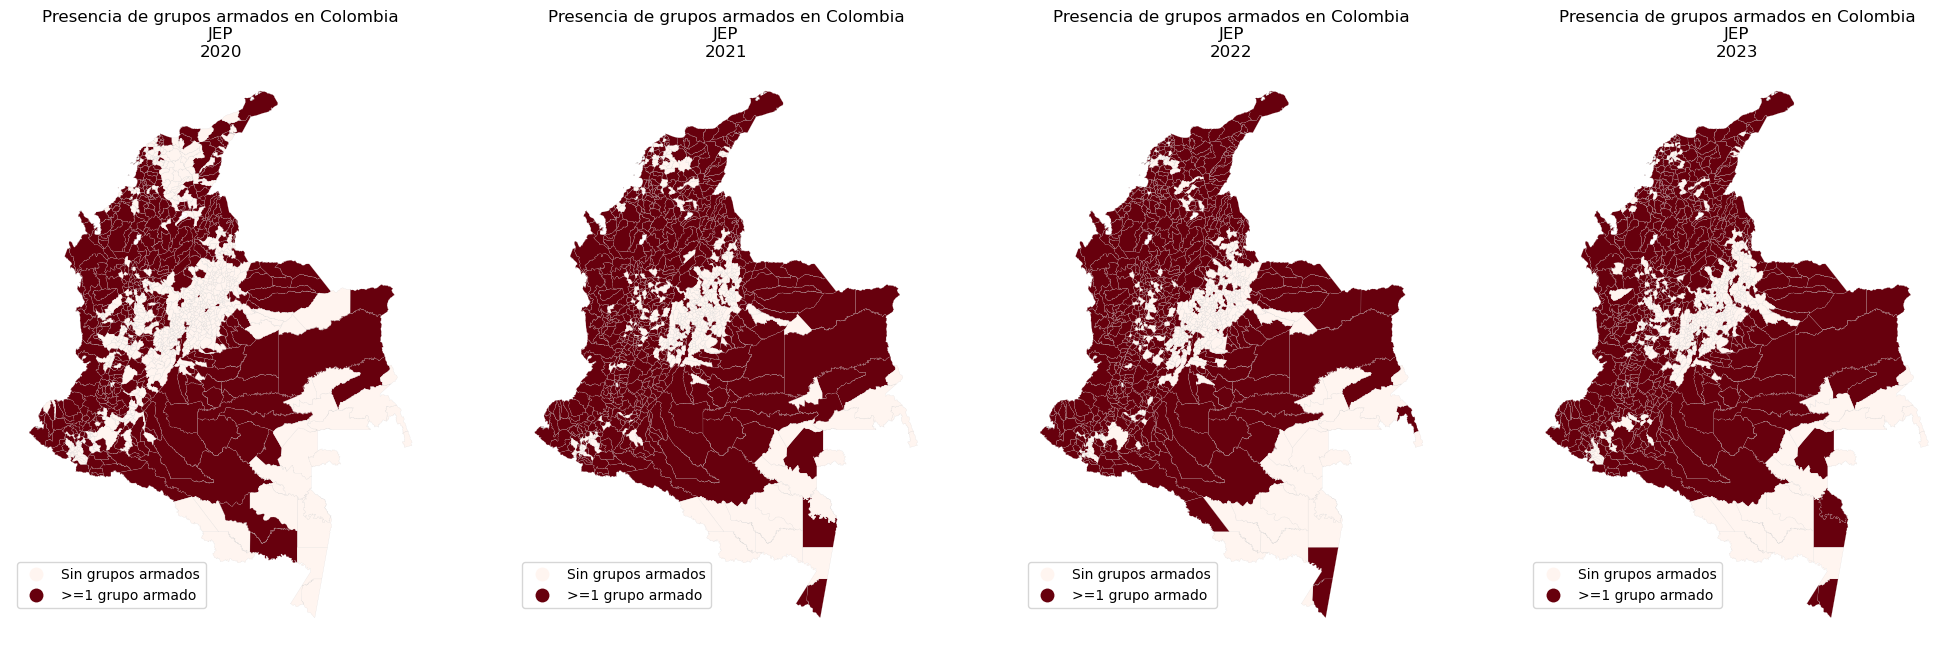
\includegraphics[width=1\textwidth, height=0.6\textheight, keepaspectratio]{Seminario de Tesis/Primera presentación/images/image.png}
        \caption{\footnotesize Expansión de grupos armados por municipios en Colombia, 2020-2023}
    \end{figure}

    \centering
    \footnotesize\textit{Fuente: Elaboración propia}
\end{frame}

\begin{frame}{Presencia de Grupos Criminales}
    \begin{figure}[ht]
        \centering
        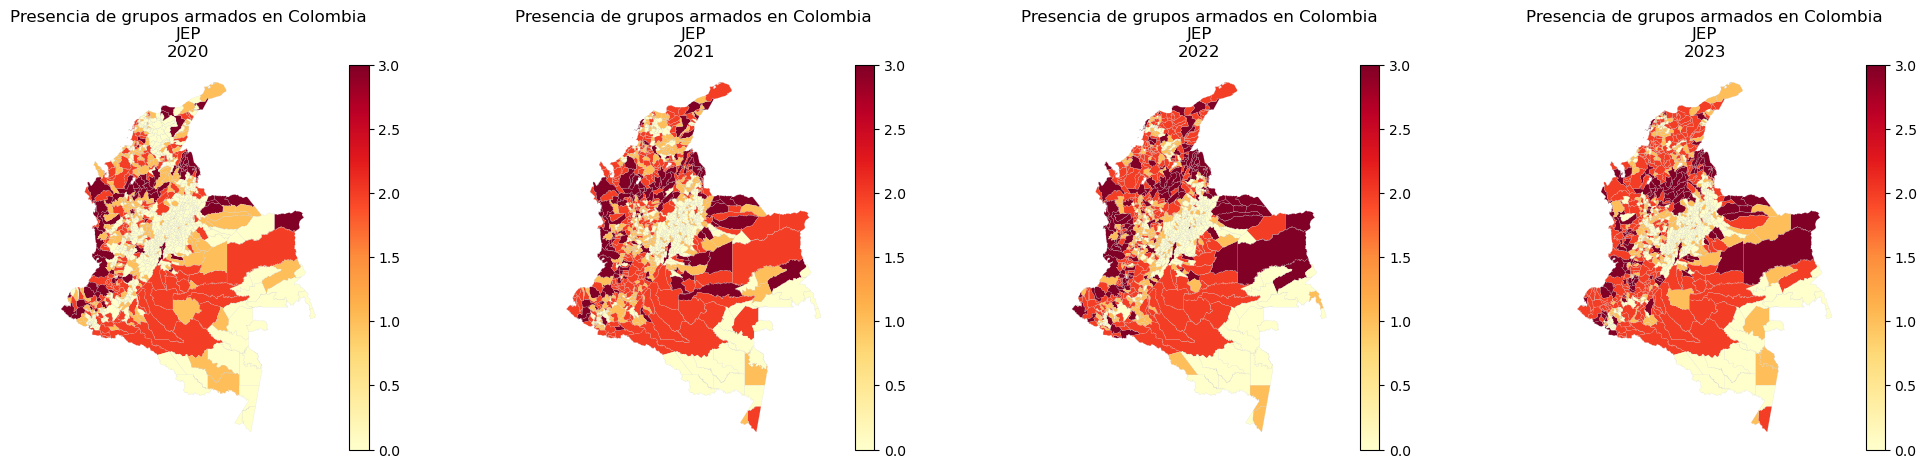
\includegraphics[width=1\textwidth, height=0.6\textheight, keepaspectratio]{Seminario de Tesis/Primera presentación/images/image 1.png}
        \caption{\footnotesize Cantidad de grupos armados por municipios en Colombia, 2020-2023}
    \end{figure}

    \centering
    \footnotesize\textit{Fuente: Elaboración propia}
\end{frame}


\begin{frame}{¿Qué definimos por violencia?}
    \pause
    \begin{block}{Índice de Violencia Agregada (IACV)}
        \begin{itemize}
            \item Componentes (Municipal y trimestral por 100,000 hab.):
            \begin{itemize}
                \item Homicidio, extorsión, secuestro, terrorismo, masacres
            \end{itemize}
            \item Ponderación por gravedad legal (Código Penal):
        \end{itemize}
        
        \centering
        \begin{tabular}{lcc}
            \toprule
            \textbf{Delito} & \textbf{Pena (años)} & \textbf{Peso (\%)} \\
            \midrule
            Homicidio & 19.0 & 17.04 \\
            Extorsión & 11.5 & 10.31 \\
            Secuestro & 16.0 & 14.35 \\
            Terrorismo & 15.0 & 13.45 \\
            Masacres & 50.0 & 44.84 \\
            \midrule
            
            \bottomrule
        \end{tabular}
        \begin{itemize}
        \item \alert{Propósito}: Medida de seguridad pública agregada
        \end{itemize}
    \end{block}

\end{frame}

\begin{frame}{¿Qué otros tipos de violencia definimos?}
    \pause
    \begin{columns}[T]
        \begin{column}{0.48\textwidth}
            \begin{block}{Índice de Amedrentamiento (IA)}
                \begin{itemize}
                    \item Componentes (Municipal y trimestral por 100,000 hab.):
                    \begin{itemize}
                        \item Amenazas
                        \item Tentativas de asesinato y atentados
                        \item Desplazamiento forzado
                        \item Hostigamiento
                    \end{itemize}
                    \item \alert{Propósito}: Medir clima de miedo
                \end{itemize}
            \end{block}
        \end{column}
        
        \begin{column}{0.48\textwidth}
            \begin{block}{Índice de Gobernanza Criminal (IGC)}
                \begin{itemize}
                    \item Componentes (Municipal y trimestral por 100,000 hab.):
                    \begin{itemize}
                        \item Confinamientos
                        \item Retenes ilegales
                        \item Paros armados
                        \item Extorsión
                    \end{itemize}
                    \item \alert{Propósito}: Medir control territorial
                \end{itemize}
            \end{block}
        \end{column}
    \end{columns}
\end{frame}

\begin{frame}{Evolución de la Violencia en Colombia}
    \begin{figure}[ht]
        \centering
        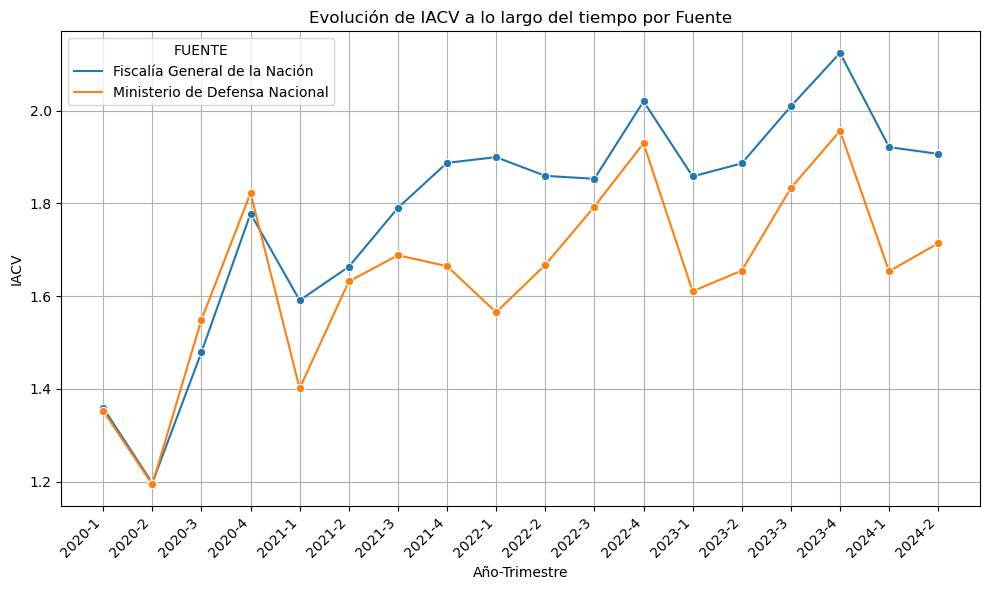
\includegraphics[width=0.9\textwidth, height=0.7\textheight, keepaspectratio]{Seminario de Tesis/Primera presentación/images/image 7.png}
    \end{figure}
    \centering
    \footnotesize\textit{Fuente: Elaboración propia}
\end{frame}

\begin{frame}{Distribución de la violencia en Colombia}
    \begin{columns}[T]
        % Columna izquierda
        \begin{column}{0.48\textwidth}
            \centering
            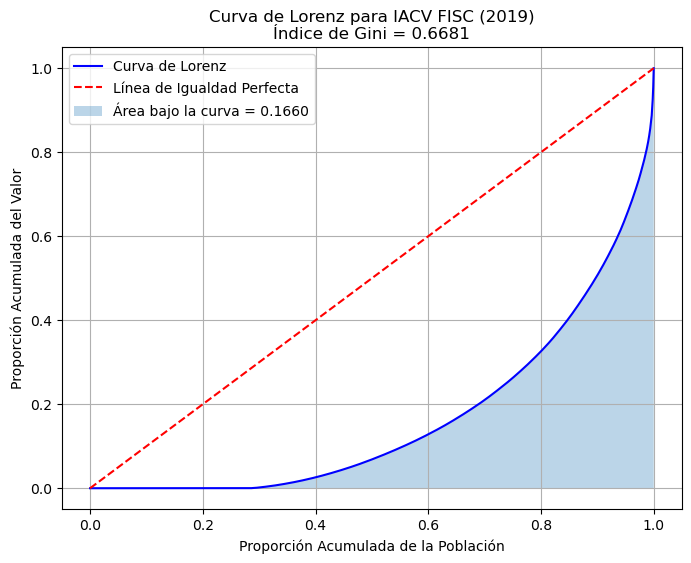
\includegraphics[width=\textwidth, height=0.65\textheight, keepaspectratio]{Seminario de Tesis/Primera presentación/images/image 3.png}
        \end{column}
        
        % Columna derecha
        \begin{column}{0.48\textwidth}
            \centering
            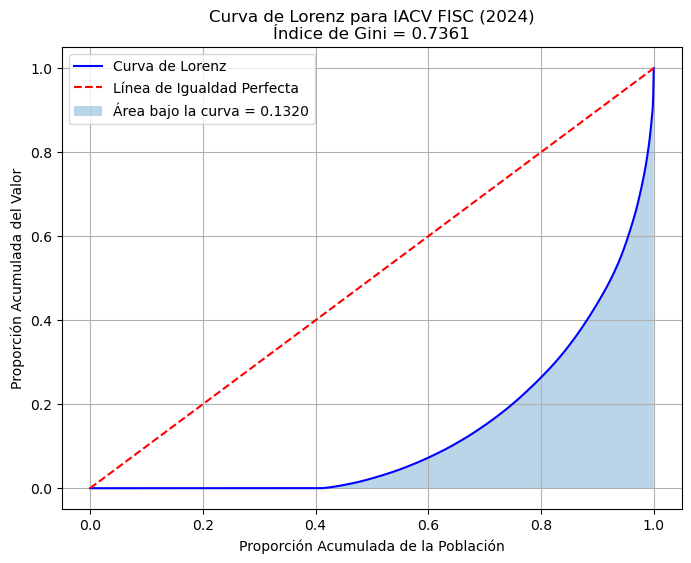
\includegraphics[width=\textwidth, height=0.65\textheight, keepaspectratio]{Seminario de Tesis/Primera presentación/images/image 4.png}
        \end{column}
    \end{columns}
    \vspace{0.2cm}
    \centering
    \footnotesize\textit{Fuente: Elaboración propia}
\end{frame}


\begin{frame}{Vulnerabilidad municipal a la violencia}
    \begin{columns}[T]
        % Columna izquierda
        \begin{column}{0.48\textwidth}
            \centering
            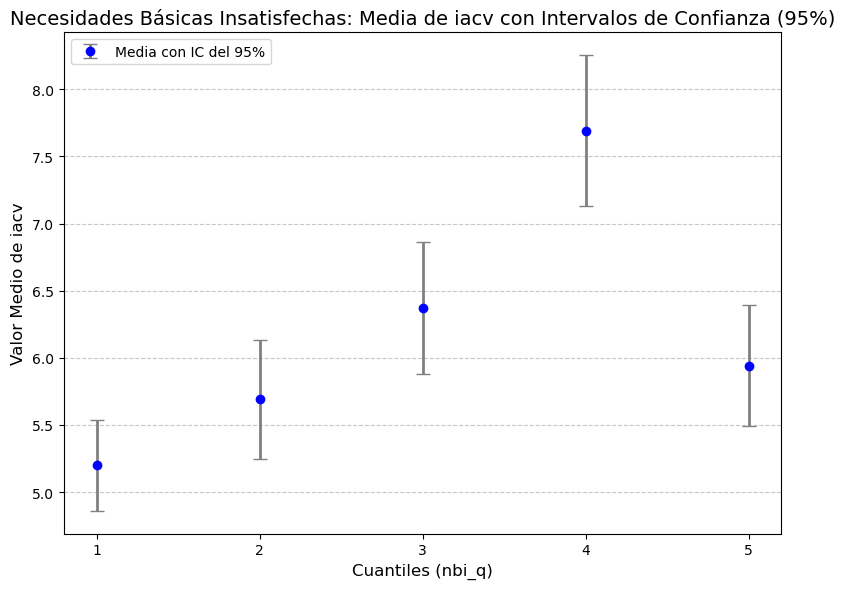
\includegraphics[width=\textwidth, height=0.65\textheight, keepaspectratio]{Seminario de Tesis/Primera presentación/images/output1.png}
        \end{column}
        
        % Columna derecha
        \begin{column}{0.48\textwidth}
            \centering
            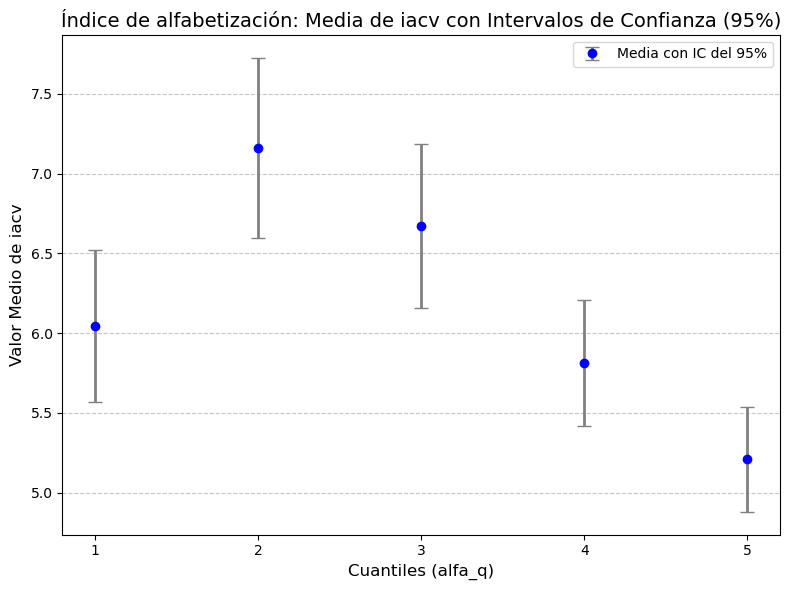
\includegraphics[width=\textwidth, height=0.65\textheight, keepaspectratio]{Seminario de Tesis/Primera presentación/images/output2.png}
        \end{column}
    \end{columns}
    \vspace{0.2cm}
    \centering
    \footnotesize\textit{Fuente: Elaboración propia}
\end{frame}